\section{Proposed VAE-accelerated EM-aware IR-drop fixing method}
\label{sec:strategy}


%In this section, we present the proposed VAE-accelerated EM-aware IR-drop fixing method. 
First we introduce our VAE-based full-chip EM-aware IR-drop prediction model, the data preparation, and training.
Then we introduce how to utilize the auto-gradient from VAE model to accelerate the convention SLP power grid fixing method ~\cite{Sukharev:2019pg}.
%We follow the notation used in~\cite{Sukharev:2019pg} to introduce the optimization frame. 
%Then we introduce our new sensitivity computation method using by VAE model.


\subsection{VAE-based EM-aware IR-drop prediction}
\label{subsec:vae}


%The Generative Adversarial Network (GAN) is a form of neural network model utilized in unsupervised machine learning, originally developed by Ian Goodfellow. A standard GAN consists of two distinct deep neural networks - the generator G and the %discriminator D. G is tasked with producing outputs closely resembling the dataset used for training, whereas D is responsible for discerning between actual and artificially generated data. The generator within a typical GAN employs a random noise vector z as %its input, converting it to output G(z). The discriminator, a deep binary classifier, accepts both genuine and manufactured data alternately, offering a "score". This score is the basis for classifying data as "authentic" or "synthetic", and is also a component of the %loss function, used to train both G and D through back propagation. Training both networks is conducted concurrently and alternately to avoid one trailing significantly behind the other until equilibrium is achieved. In comparison, a regular Convolutional Neural %Network (CNN) utilizes a simple least square loss function, whereas the loss function of a GAN is a combination of the least square loss between prediction and actual data, and a discriminator's score. Thus, a GAN can be perceived as an advanced CNN with %improved accuracy.

%The Conditional Generative Adversarial Network (CGAN) operates within conditional settings, learning a conditional generative model. In contrast to a standard GAN, the generator's input in a CGAN is a fusion of both a condition vector x and a random noise %vector z, with the output labelled as G(x, z). The fundamental disparity with GAN lies in the fact that both G and D in a CGAN are conditional on vector x. CGANs have demonstrated outstanding performance in image-to-image translation tasks, where the input %image acts as the condition, directing the image generation process. In our study, the EM stress distribution generated is contingent on the input current density and given aging time, following the physics-law of stress evolution, making the CGAN model %exceptionally suitable.

The traditional autoencoder(AE) structure includes encoder and decoder structures. A input will be encoded to a determined latent variable by the encoder, and then decoded to the output by the decoder.  The GAN model adopts the standard autoencoder to generate the result, and use an additional binary output CNN as the discriminative network only in the training stage to better train the autoencoder. 
 
Variational autoencoder (VAEs) is a type of unique generative model derived from the standard autoencoder, which are used to generate new data that is similar to the input data they're trained on. 
Compared to traditional autoencoder structure, VAE does not directly encode the input to a determined latent variable, instead its encoded to a distribution over the latent space,  and then re-samples from this distribution to generate a latent variable for the decoder. This re-sampling step is crucial to the VAE's some crucial characteristics over GANs, such as Interpretability of Latent Space, and Training Stability.
Interpretability of Latent Space means that the latent space is smooth and interpretable, enabling nice properties like the ability to interpolate between different points in the latent space and generate new samples that exhibit a smooth transition between the characteristics of the original points. On the other hand, GANs do not explicitly enforce such a structure, making the latent space less interpretable and interpolations might not always produce meaningful outputs. 

The Loss function for a VAE has two parts. The first is the reconstruction loss, which encourages the decoded output data to be similar to the label. As our data is continuous, we apply the mean squared error (MSE) for the reconstruction loss evaluation.
The second part is the Kullback-Leibler (KL) divergence between the latent variable distribution $Q(z|x)$ output by the encoder and a chosen prior distribution, usually a standard multivariate Gaussian distribution $\mathcal{N}(\textbf{0}, \textbf{I})$. The KL divergence measures how one probability distribution is different from a second, which acts as a regularization term to force the encoded latent distribution from the given training dataset to be close to a standard normal distribution, and encourage the network to use the latent space efficiently. 
For each datapoint x, if we denote the mean of $Q(z|x)$ as $\mu$ and the standard deviation as $\sigma$, this loss can be written as:
%$\mathcal{N}(\mu_{x}, \sigma_{x}^{2})$ 

\begin{equation}
	\label{eq:vae_KLD_loss}
	D_{KL}( \mathcal{N}(\mu_{x}, \sigma_{x}^{2}) ~ || ~ \mathcal{N}(\textbf{0}, \textbf{I} ) )  = \dfrac{1}{2} (-\log\sigma^{2} + \mu^{2} + \sigma^{2} - 1)
\end{equation}

During training, the VAE learns to map the input data to a lower-dimensional latent space in a way that it can generate similar data from points in this space. Because of the probabilistic nature of the encoding, and the use of the KL divergence in the loss function, the VAE is encouraged to create a smooth and continuous latent space, where similar points decode to similar data.
\begin{equation}
	\label{eq:vae_total_loss}
	%\min_{\theta}  \{  \textit{MSE} (y , \hat{y} )   ~ + ~  D_{KL}( \mathcal{N}(\mu_{x}, \sigma_{x}^{2}) ~ || ~ \mathcal{N}(\textbf{0}, \textbf{I} ) )  \}
	\min  \{  \textit{MSE} (y , \hat{y} )   ~ + ~  D_{KL}( \mathcal{N}(\mu_{x}, \sigma_{x}^{2}) ~ || ~ \mathcal{N}(\textbf{0}, \textbf{I} ) )  \}
\end{equation}

\begin{figure*}[h!]
	\centering
	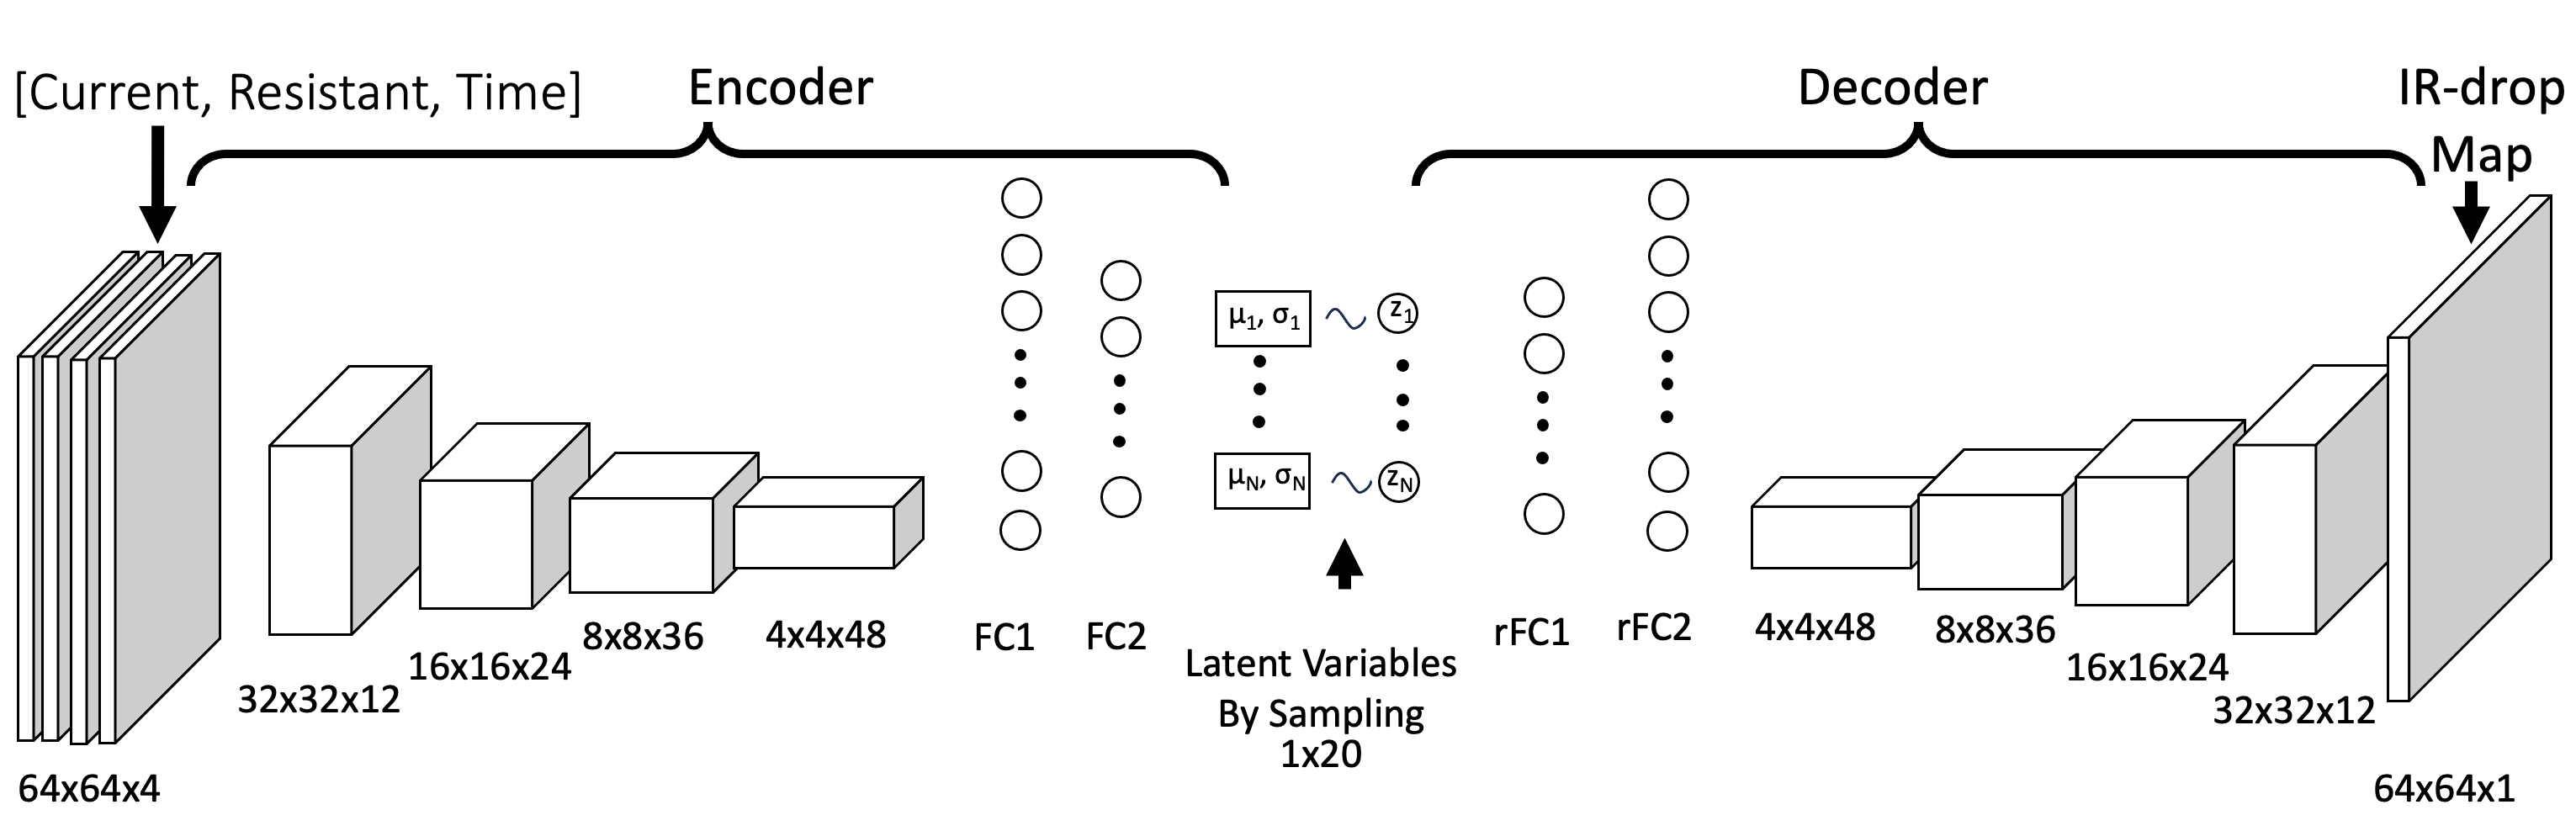
\includegraphics[width=1.8\columnwidth]{./figs/VAE_temp.eps}
	\caption{The VAE model structure in our method} 
	\label{fig:VAE_architecture}
\end{figure*}

The inputs include power grid conductance matrix \textit{\textbf{G}}, the current source drawn from it to other circuit layers, and a target life time \textit{\textbf{t}} as the conditional information. 
The VAE model contain four convolutional layers and two fully-connected layers. The input is first padded to the standard size of 64 x 64 for the power grid smaller than this size. If the power grid exceeds the size of 64 x 64 but smaller than 128 x 128, then we add one more convolutional layer in both the generator and the discriminator network. For the further larger or smaller sized power grid, we follow the same routine to add or remove the convolutional layers to fit the input size.

As for our VAE-based model training, first we extract the electrical information from the result of the  $\it{EMspice}$. The input features of VAE model should include the node voltage $u(t)$ and $M(t)$,  the conductance matrix of the power grid network.
%in the format of wire segment resistance vectors, which are mentioned in Eq.~\eqref{eq:mna}. 


The data preprocessing before the model training is as follows. Synopsys IC compiler can automatically create the circuit layout from a synthesized gate-level netlist and a standard cell library. 
Then we parse the electrical features and the topological information from the circuit layout.

\begin{table}[!htbp]
	\begin{center}
		\caption{Power Grid Design Detail}
		\label{table:pre_results}
		%\vspace{-0.1in}
		\center
		\resizebox{0.48\textwidth}{!}{
		\begin{tabular}{ c | c | c | c | c}
			\hline 
			circuit &{\# nodes}&{\# Trees}&{\# voltage sources} &{$V_{DD}$ (V)}  \\ \hline 
			\hline 
			Design1 &1024 &64   &4 &1.05  \\ \hline
			Design2 &4096 &128  &4 &1.05 \\ \hline
			Design3 &16384 &256 &4 &1.05  \\ \hline
		\end{tabular}
		}
	\end{center}
	\vspace{-0.1in}
\end{table}

\begin{table}[!h]
	\begin{center} 
		\caption{Prediction results of VAE model and GAN model on different designs}
		\label{table: Model_RMSE_Compare}
		\center
			\begin{tabular}{| c| c | c | c | }
				\hline 
				{} &{} &\multicolumn{2}{c|} {RMSE (mV)}  \\
				\cline{3-4}
				\multirow{-2}{*}{Circuit}   &\multirow{-2}{*}{\# nodes} &{ GAN}  &{ VAE}   \\ \hline 
				\hline 
				Design1  &1024      &5.697 	& 3.144 	 \\ \hline
				Design2  &4096      &6.100	&  3.519	\\ \hline
				Design3  &16384   &3.922	        &  3.462	\\ \hline			
			\end{tabular}
	\end{center}
	\vspace{-0.1in}
\end{table}





\subsection{power grid EM-aware IR-drop failure fixing framework }
\label{subsec:formulation}

The structure of the combined VAE and  $\it{EMspice}$ analysis of the proposed strategy is shown in Fig.~\ref{subfig:flow-framework}. The workflow is concluded in Fig.~\ref{subfig:flow}. 

\begin{figure*}[h!]
	\centering
	\captionsetup{justification=centering, margin=3cm}
	\subfigure[]{
		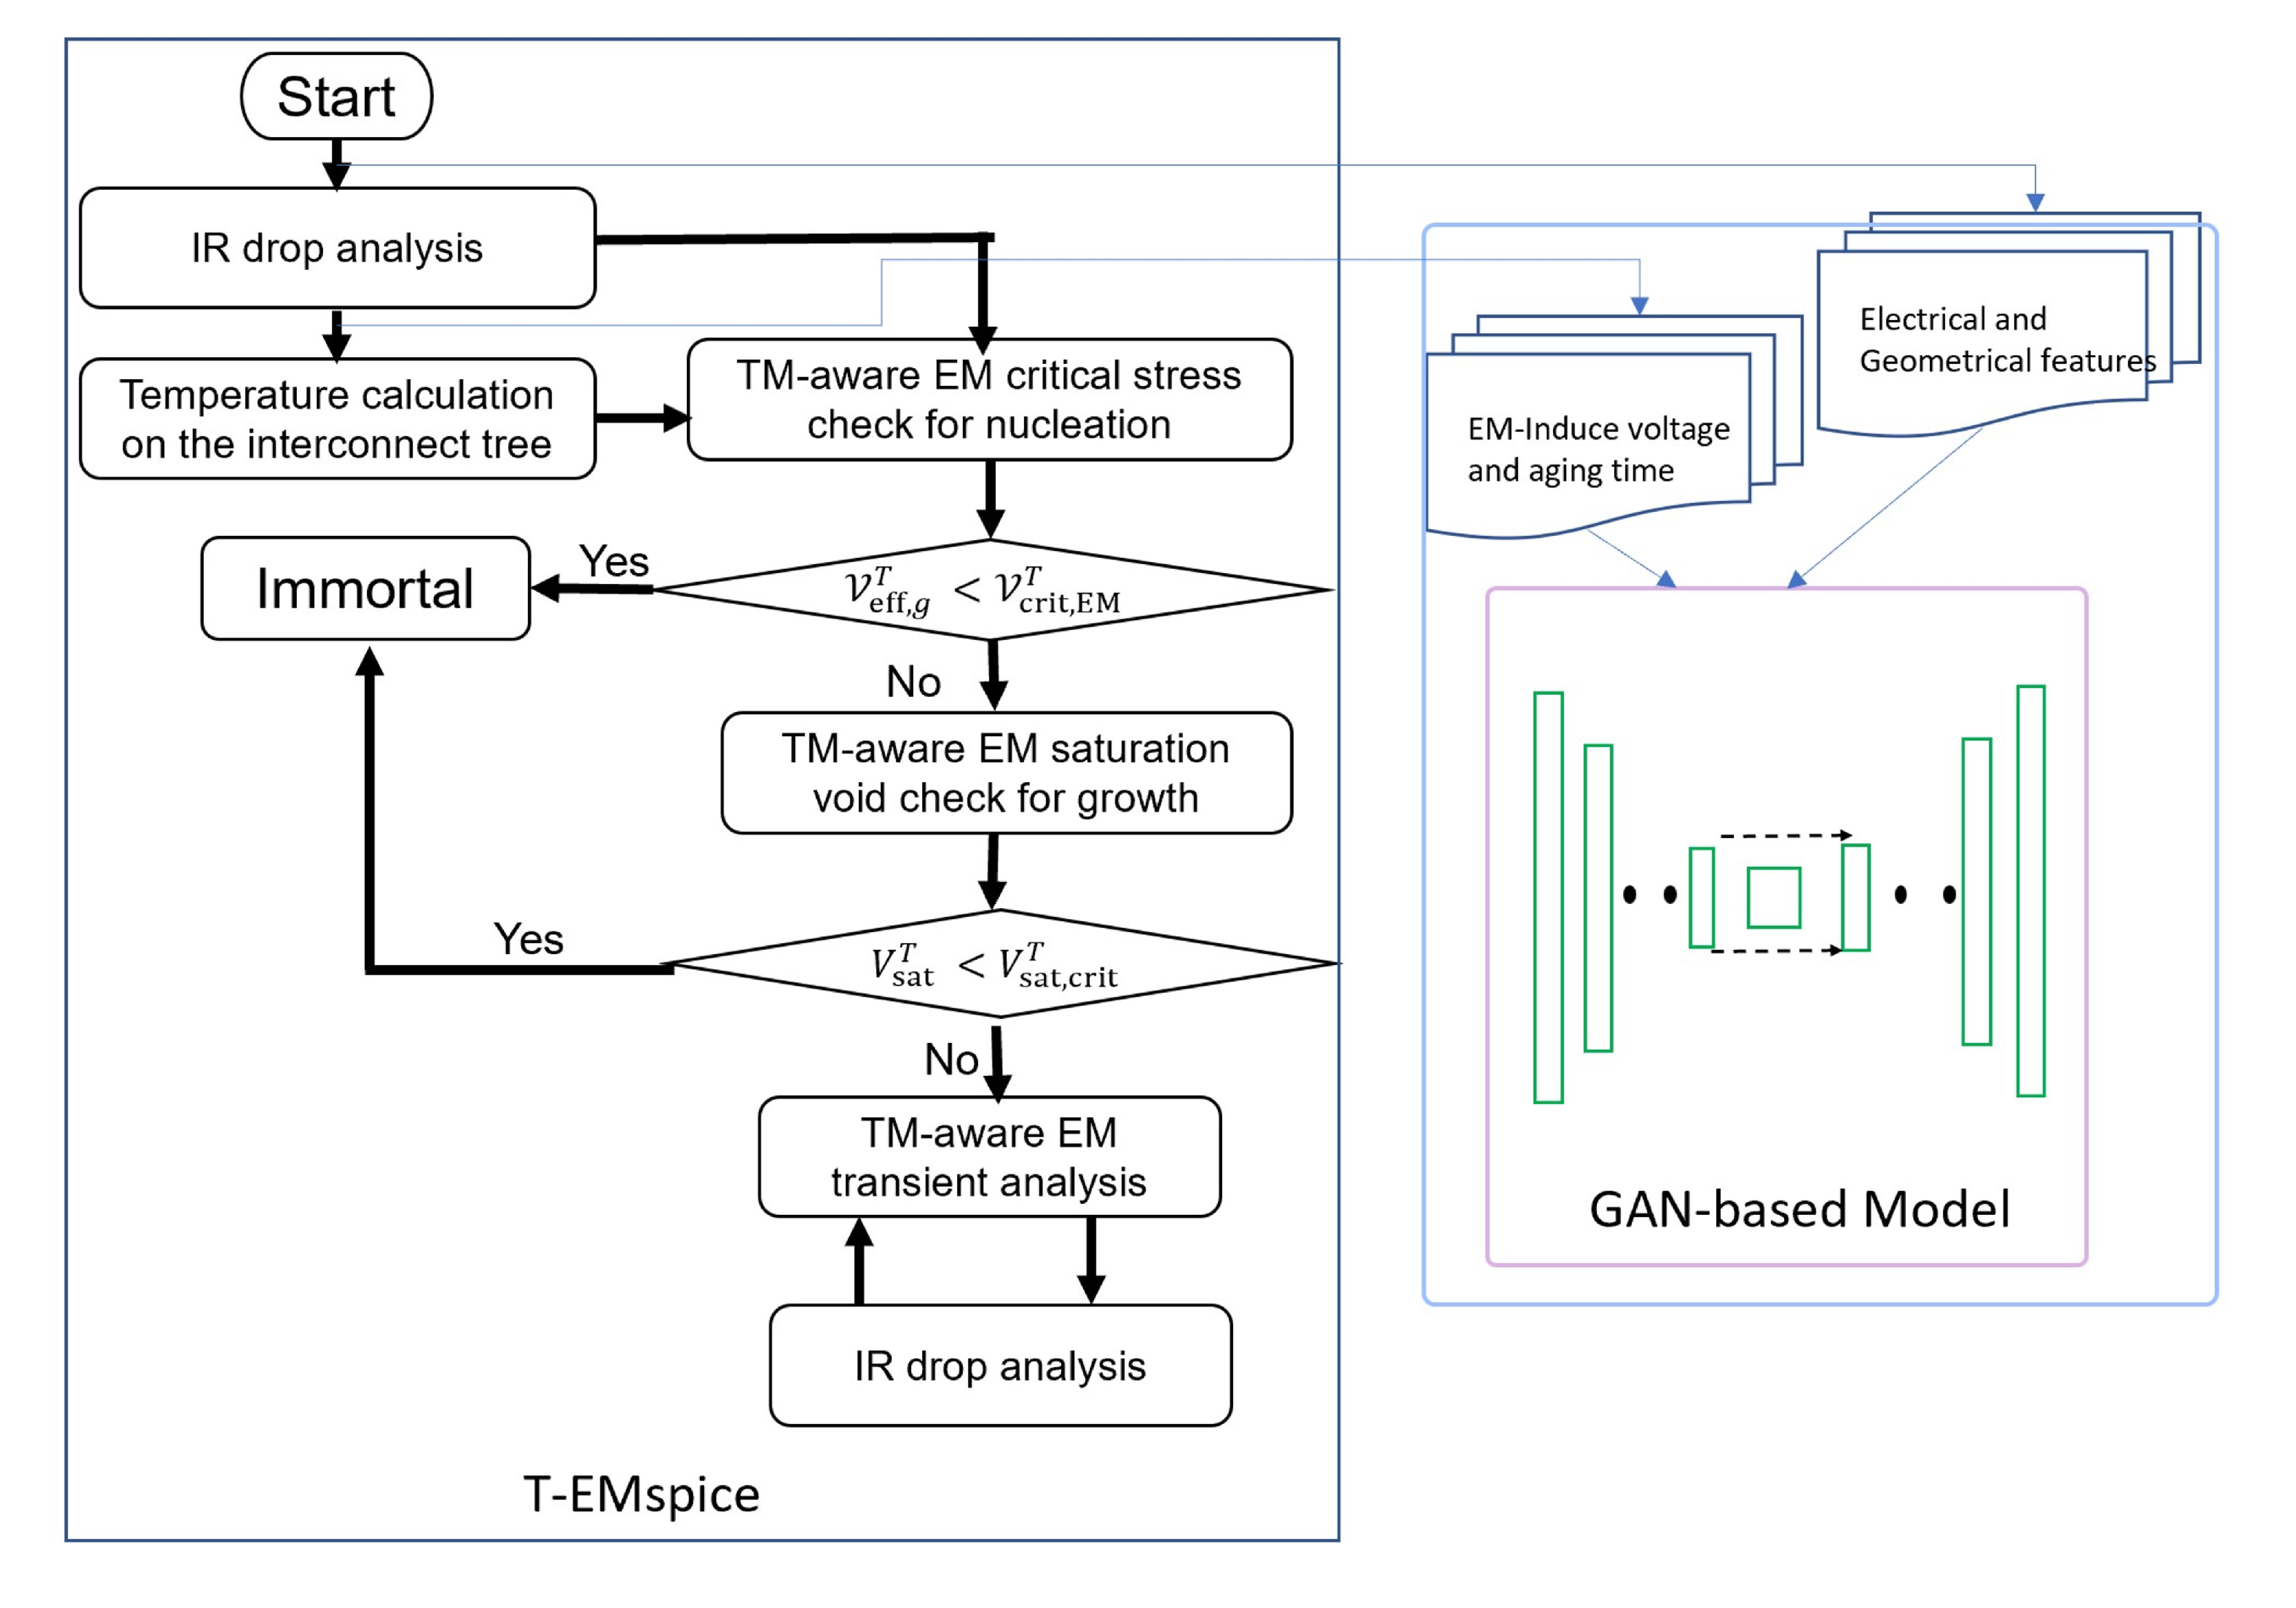
\includegraphics[width=1.207\columnwidth]{./figs/flow.eps}
		\label{subfig:flow-framework}}
	\subfigure[]{
		\includegraphics[width=0.74\columnwidth]{./figs/workflow-gridnetslp.eps}
		\label{subfig:flow}}
	\caption{The proposed (a)framework of  VAE-accelerated power gird fixing method (b) workflow of the fixing method.}
	\label{fig:flow}
\end{figure*}



\subsubsection{problem formulation}
\label{subsubsec:formulation}
The proposed method intends to solve the following problem: 
Given the power grid information at T=0, our VAE-based model has predict the EM-aware IR-drop the target aging life time \textit{\textbf{t}} in ~\ref{subsec:vae}.The power grid has EM-induced IR drop violations and demands fixing if it has node voltage drop \textit{\textbf{v}}  above the threshold $V_{th}$.
We wish to alleviate the EM-aware IR drop failure by resizing the power grid interconnect trees width with minimum metal area increase.

The problem can be formulated as:
\begin{align}
	\label{eq:prob_formulation}
	&\mbox{Minimize}  & a^{t}s \qquad   \notag  \\
	&s.t.     & v(t,s)\leq V_{th} \\
	& \quad   &s \in S   \triangleq \{ s \in R^{nt}: 1 \leq s \leq s_{up} \}        \notag
\end{align}

In \eqref{eq:prob_formulation}, $a=[a_{1},a_{2},\ldots,a_{nt}] = [w_{1}l_{1},w_{2}l_{2},\ldots,w_{nt}l_{nt}]$ refers to the metal areas of power grid with $n_{t}$ trees, $w_{i}$ and $l_{i}$ are the $i_{th}$ tree's width and length separately.
For the constraints, $s=[s_{1},s_{2},\ldots,s_{nt}]$  is the resizing factor for the power grid trees. $S$ is the feasible region ,
where $s_{up}$ is the upper bound for $s$. Similar to~\cite{Sukharev:2019pg}, we assume the original power grid trees are already set to its minimum width. Hence we only increase the tree width and $s \geq 1 $.
The feasible region reflects both the basic design rules and case-by-case user requirements, such as the criteria of minimum interconnect tree width, the minimum spacing to prevent the  interconnect trees overlap, and the maximum metal area usage, etc. 
The node IR drop $v(t,s)$  is the voltage difference between the power grid interconnect node and the power supply, its is a nonlinear function to $s$ at aging time $t$. The maximum allowable voltage drop threshold $V_{th}$ is given by user, we assumed it to be ten percents of the power supply voltage.


\subsubsection{Programming-based optimization}
\label{subsubsec:slp_framework}

As we mentioned in ~\ref{subsubsec:formulation}, the EM-aware PG node voltage drop $v(t,s)$ is a nonlinear function to $s$ at aging time $t$, hence \eqref{eq:prob_formulation} is a nonlinear optimization problem. 
We solve it by a stepping strategy, which we linearize the voltage drop at current latest solution point by Taylor's expansion \eqref{eq:v_taylor_expand} , and solve it with linear programming (LP) solver. We repeat this operation until the power grid has no EM-aware IR drop violation.

\begin{equation}
	\label{eq:v_taylor_expand}
	v(t, s^{(i+1)}) \triangleq v(t,s^{(i)}) + \dfrac{\partial v(t, s^{(i)})}{\partial s} \cdot \delta s
\end{equation}
where $s^{(i)}$ denotes the current power grid resizing vector and $s^{(i+1)}$ is defined as 
\begin{equation}
	\label{eq:s}
	s^{(i+1)} = s^{(i)} + \delta s 
\end{equation}

$ \dfrac{\partial v(t, s)}{\partial s}$ is the $n\times n_{t}$ \textit{Jacobian} matrix of $v(t,s)$ with respect to $s$, describes how the node voltage drops at target time $T=t$ respond to the corresponding tree width rescaling.

\begin{equation}
	\label{eq:J_matrix}
	\dfrac{\partial v(t, s)}{\partial s}=
	\mathbf {J}_{n\times n_{t}}(s,t) =
	\begin{bmatrix}
		\frac{\partial v(1,t)}{\partial s_{1}}&\frac{\partial v(1,t)}{\partial s_{2}}&\ldots&\frac{\partial v(1,t)}{\partial s_{n_{t}}}\\
		\frac{\partial v(2,t)}{\partial s_{1}}&\frac{\partial v(2,t)}{\partial s_{2}}&\ldots&\frac{\partial v(2,t)}{\partial s_{n_{t}}}\\
		\vdots&\vdots&\ddots&\vdots\\
		\frac{\partial v(n,t)}{\partial s_{1}}&\frac{\partial v(n,t)}{\partial s_{2}}&\ldots&\frac{\partial v(n,t)}{\partial s_{n_{t}}}
	\end{bmatrix}
\end{equation}



\subsubsection{Fast Gradient acquisition}
PyTorch auto differentiation can provide the gradient of output node voltages to the input wire segment conductances, which is $ \dfrac{\partial v(t, s)}{\partial g}$. Then we can easily get \eqref{eq:J_matrix} by chain rule, as each power grid tree $g_{i}$ has its own resizing factor $s_{i}$ and will not be infected by other resizing factors:
\begin{equation}
	\label{eq:chain_rule}
	\begin{aligned}
	\begin{split}
	\frac{\partial v}{\partial s} & =\frac{\partial v}{\partial g} \frac{\partial g}{\partial s}, \\ 
	\frac{\partial g_{i}}{\partial s_{k}} & = 
    	\begin{cases}
        		0,      &\mbox{if i $\neq$ k} \\ 
        		g_{i},  &\mbox{if i = k} 
    	\end{cases}
	\end{split}
	\end{aligned}
\end{equation}



As Comparison, we compare to the sensitivity ~\cite{Sukharev:2019pg}
For a the power grid network represented by the node conductance matrix $ \textit{G(t,s)}$, we can write its model in the format of the following equation:
\begin{equation}
	\label{eq:gv=i}
	G(t,s)\cdot v(t,s)= j(t)
\end{equation}
where $j(t)$  is $n\times 1$ vectors representing and node current vector for the power grid.

And the sensitivity 
\begin{equation}
	\label{eq:dVs}
	\dfrac{\partial v(t,s)}{\partial s_{k}} = -G^{-1}\cdot \dfrac{\partial G(t,s)}{\partial s_{k}}  \cdot G^{-1}\cdot j(t)
\end{equation}




To solve the above equation and obtain $ \frac{\partial v(t,s)}{\partial s_{k}}$, one has to first construct the G-related matrices , and then perform expensive computational matrix solving. 

%first we obtain $x = G^{-1}(t,s) \cdot j(t)$ by solving 
 %\begin{equation}
%   G(t,s) \cdot x = j(t)
%   \label{eq:solving1}
%\end{equation}
%Then we calculate $y = \dfrac{\partial G(t,s)}{\partial s_{k}} \cdot x$. After this we solve the following equation again
%\begin{equation}
%	G(t,s) \cdot \dfrac{\partial v(t,s)}{\partial s_{k}} = y
%	\label{eq:solving2}
%\end{equation}

%As we can see, we need to perform matrix solving twice in \eqref{eq:solving1} and \eqref{eq:solving2} for {\it each} power grid tree $k$. 
Even if we only need to do one LU factorization on $G$ matrices for each $s$ value, we still need to solve back-substitutions each time for \eqref{eq:solving1} and \eqref{eq:solving2} . These are very expensive computations especially when the number of violations nodes and trees are large ($k$ is larger).
Notice that the circuit node conductance matrix $G(t,s)$ is a sparse matrix. The sparsity remains in all the derived matrices of $G(t,s)$, such as $\dfrac{\partial G(t,s)}{\partial s_{k}}$ for all $k$.
Thereby the circuit matrix-based method not only suffers a large computation workload during the matrix solving procedure but also undertakes a large time consumption for the circuit matrix construction as $G(t,s)$ and its derived matrices increases quadratically over the power grid node size $n$. In this work, we try to mitigate these issues by using DDN based modeling, which is much more scalable with the size of power gird and the number of violation, as will show soon in the next section. 


Notice that each column of \eqref{eq:J_matrix} has to be calculated through the entire process described in \eqref{eq:dVs} for the corresponding power grid tree. In comparison our VAE-based method constructs the \textit{Jacobian} matrix by conducting the inference procedure only once.





%We utilize the auto differentiation to calculate the sensitivity of output node voltage to the input power grid wire segment resistance, as VAE models are differentiable with respect to the model parameters. 
%First we train the VAE model extracted from the analytical results from $\it{EMspice}$, which provides the node voltage and branch resistance information of the power grid from $T = 0$ to $T = T_{target}$. 


%The output of the VAE mode contains two parts, the first part is the power grid nodes voltage at the target aging time considering the EM-induced aging effect, the second part is the sensitivity(gradient) of the output (voltage) with respect to the inputs (such as the resizing factor $s_{k}$ for the $k_{th}$ tree).  Such gradient acquisition can be very efficient as we can compute all the sensitivities just by one back propagation, and all the local gradients have been computed already. The acquirement of such sensitivity in our method utilizes the inherent characteristics of the differentiable VAE model. Once the models have been trained, they have the promise to be applied to the different designs, specially by using localized training as shown in recent work~\cite{WenPan:SemiTherm'2020}. 








